\documentclass[tikz,border=5pt]{standalone}
\usepackage[T1]{fontenc}
\usepackage{lmodern,amsmath,amssymb}
\usetikzlibrary{arrows.meta,calc,positioning,fit,backgrounds,shapes.geometric,matrix,decorations.pathreplacing,patterns}
\definecolor{ink}{gray}{0.08}
\definecolor{wash}{gray}{0.965}
\definecolor{soft}{gray}{0.45}
\tikzset{box/.style={draw=ink,line width=.65pt,fill=white,align=center,inner sep=4pt,outer sep=0pt,font=\small},flow/.style={draw=ink,line width=.65pt,-{Latex[length=1.8mm,width=1.3mm]},rounded corners=2pt},annotation/.style={font=\scriptsize,text=soft,align=center},groupbox/.style={draw=soft,dashed,line width=.45pt,fill=wash}}
\begin{document}
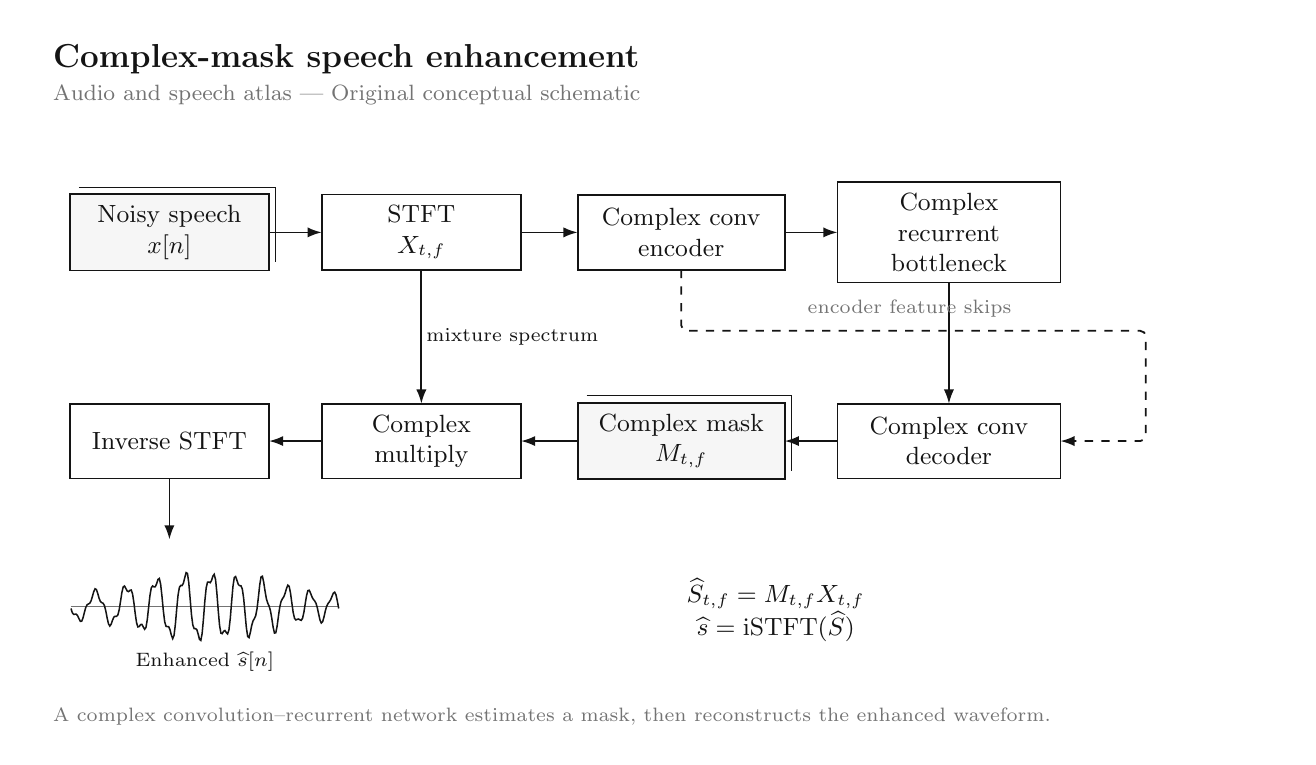
\begin{tikzpicture}[x=1cm,y=-1cm,font=\rmfamily,text=ink]

\path[use as bounding box] (0,0) rectangle (16,9);
\node[anchor=west,font=\large\bfseries] at (.2,.4) {Complex-mask speech enhancement};
\node[anchor=west,font=\footnotesize,text=soft] at (.2,.85) {Audio and speech atlas | Original conceptual schematic};
\begin{pgfonlayer}{background}
\end{pgfonlayer}
\node[box,fill=wash,minimum width=2.5cm,minimum height=0.95cm,text width=2.25cm] (noisy) at (1.8,2.6) {Noisy speech\\$x[n]$};
\draw[ink,line width=.4pt] (0.65,2.025) -- (3.15,2.025) -- (3.15,2.975);
\node[box,minimum width=2.5cm,minimum height=0.95cm,text width=2.25cm] (stft) at (5.0,2.6) {STFT\\$X_{t,f}$};
\node[box,minimum width=2.6cm,minimum height=0.95cm,text width=2.35cm] (encoder) at (8.3,2.6) {Complex conv\\encoder};
\node[box,minimum width=2.8cm,minimum height=0.95cm,text width=2.55cm] (rnn) at (11.7,2.6) {Complex recurrent\\bottleneck};
\node[box,minimum width=2.8cm,minimum height=0.95cm,text width=2.55cm] (decoder) at (11.7,5.25) {Complex conv\\decoder};
\node[box,fill=wash,minimum width=2.6cm,minimum height=0.95cm,text width=2.35cm] (mask) at (8.3,5.25) {Complex mask\\$M_{t,f}$};
\draw[ink,line width=.4pt] (7.1000000000000005,4.675000000000001) -- (9.700000000000001,4.675000000000001) -- (9.700000000000001,5.625);
\node[box,minimum width=2.5cm,minimum height=0.95cm,text width=2.25cm] (product) at (5.0,5.25) {Complex\\multiply};
\node[box,minimum width=2.5cm,minimum height=0.95cm,text width=2.25cm] (istft) at (1.8,5.25) {Inverse STFT};
\begin{pgfonlayer}{background}
\draw[flow] (noisy.east) -- (stft.west);
\draw[flow] (stft.east) -- (encoder.west);
\draw[flow] (encoder.east) -- (rnn.west);
\draw[flow] (rnn.south) -- (decoder.north);
\draw[flow] (decoder.west) -- (mask.east);
\draw[flow] (mask.west) -- (product.east);
\draw[flow] (product.west) -- (istft.east);
\draw[flow] (stft.south) -- (product.north) node[midway,right,fill=white,inner sep=1.5pt,font=\scriptsize] {mixture spectrum};
\draw[flow,dashed] (encoder.south) -- (8.3,3.85) -- (14.2,3.85) -- (14.2,5.25) -- (decoder.east);
\end{pgfonlayer}
\node[align=center,anchor=center,font=\scriptsize,text=soft,text width=5.5cm] at (11.2,3.57) {encoder feature skips};
\draw[soft,line width=.35pt] (0.55,7.35) -- (3.95,7.35);
\draw[ink,line width=.55pt] plot coordinates {(0.550,7.376) (0.567,7.430) (0.584,7.451) (0.601,7.449) (0.618,7.449) (0.635,7.469) (0.652,7.507) (0.669,7.539) (0.686,7.538) (0.703,7.495) (0.720,7.428) (0.737,7.365) (0.754,7.330) (0.771,7.319) (0.788,7.310) (0.805,7.280) (0.822,7.224) (0.839,7.162) (0.856,7.126) (0.873,7.136) (0.890,7.186) (0.907,7.246) (0.924,7.288) (0.941,7.302) (0.958,7.310) (0.975,7.339) (0.992,7.406) (1.009,7.495) (1.026,7.570) (1.043,7.599) (1.060,7.576) (1.077,7.527) (1.094,7.487) (1.111,7.475) (1.128,7.477) (1.145,7.459) (1.162,7.394) (1.179,7.287) (1.196,7.176) (1.213,7.103) (1.230,7.091) (1.247,7.122) (1.264,7.155) (1.281,7.162) (1.298,7.146) (1.315,7.142) (1.332,7.191) (1.349,7.302) (1.366,7.442) (1.383,7.558) (1.400,7.611) (1.417,7.605) (1.434,7.580) (1.451,7.579) (1.468,7.610) (1.485,7.640) (1.502,7.618) (1.519,7.518) (1.536,7.363) (1.553,7.210) (1.570,7.114) (1.587,7.090) (1.604,7.102) (1.621,7.100) (1.638,7.061) (1.655,7.007) (1.672,6.995) (1.689,7.070) (1.706,7.225) (1.723,7.406) (1.740,7.544) (1.757,7.603) (1.774,7.607) (1.791,7.608) (1.808,7.647) (1.825,7.716) (1.842,7.759) (1.859,7.717) (1.876,7.575) (1.893,7.379) (1.910,7.205) (1.927,7.107) (1.944,7.084) (1.961,7.085) (1.978,7.055) (1.995,6.985) (2.012,6.921) (2.029,6.931) (2.046,7.050) (2.063,7.248) (2.080,7.451) (2.097,7.585) (2.114,7.632) (2.131,7.632) (2.148,7.644) (2.165,7.700) (2.182,7.768) (2.199,7.782) (2.216,7.691) (2.233,7.502) (2.250,7.282) (2.267,7.115) (2.284,7.042) (2.301,7.040) (2.318,7.049) (2.335,7.021) (2.352,6.966) (2.369,6.942) (2.386,7.009) (2.403,7.180) (2.420,7.402) (2.437,7.591) (2.454,7.689) (2.471,7.696) (2.488,7.666) (2.505,7.656) (2.522,7.681) (2.539,7.699) (2.556,7.649) (2.573,7.503) (2.590,7.293) (2.607,7.097) (2.624,6.983) (2.641,6.971) (2.658,7.021) (2.675,7.071) (2.692,7.087) (2.709,7.088) (2.726,7.129) (2.743,7.247) (2.760,7.430) (2.777,7.616) (2.794,7.732) (2.811,7.746) (2.828,7.680) (2.845,7.593) (2.862,7.534) (2.879,7.505) (2.896,7.467) (2.913,7.379) (2.930,7.235) (2.947,7.078) (2.964,6.975) (2.981,6.967) (2.998,7.045) (3.015,7.159) (3.032,7.254) (3.049,7.309) (3.066,7.346) (3.083,7.403) (3.100,7.500) (3.117,7.612) (3.134,7.688) (3.151,7.685) (3.168,7.600) (3.185,7.472) (3.202,7.355) (3.219,7.284) (3.236,7.252) (3.253,7.227) (3.270,7.182) (3.287,7.122) (3.304,7.080) (3.321,7.096) (3.338,7.181) (3.355,7.307) (3.372,7.427) (3.389,7.501) (3.406,7.522) (3.423,7.514) (3.440,7.510) (3.457,7.520) (3.474,7.527) (3.491,7.500) (3.508,7.425) (3.525,7.316) (3.542,7.211) (3.559,7.149) (3.576,7.145) (3.593,7.182) (3.610,7.228) (3.627,7.259) (3.644,7.279) (3.661,7.308) (3.678,7.365) (3.695,7.445) (3.712,7.522) (3.729,7.561) (3.746,7.545) (3.763,7.484) (3.780,7.408) (3.797,7.348) (3.814,7.314) (3.831,7.292) (3.848,7.264) (3.865,7.222) (3.882,7.181) (3.899,7.169) (3.916,7.204) (3.933,7.283) (3.950,7.376)};
\draw[flow] (1.8,5.73) -- (1.8,6.5);
\node[align=center,anchor=center,font=\scriptsize,text=ink,text width=4cm] at (2.25,8.05) {Enhanced \mbox{$\widehat{s}[n]$}};
\node[align=center,anchor=center,font=\small,text=ink,text width=9cm] at (9.5,7.4) {\mbox{$\widehat{S}_{t,f}=M_{t,f}X_{t,f}$}\\\mbox{$\widehat{s}=\operatorname{iSTFT}(\widehat S)$}};
\node[anchor=west,align=left,font=\scriptsize,text=soft,text width=15.6cm] at (.2,8.75) {A complex convolution--recurrent network estimates a mask, then reconstructs the enhanced waveform.};
\end{tikzpicture}
\end{document}
